\documentclass[11pt]{article}
\usepackage[utf8]{inputenc}
\usepackage[T1]{fontenc}
\usepackage[spanish,es-noshorthands]{babel}
\usepackage[margin=2.5cm]{geometry}
\usepackage{amsmath,amssymb}
\usepackage{graphicx}
\usepackage{booktabs}
\usepackage{xcolor}
\usepackage[colorlinks=true,linkcolor=blue,citecolor=blue,urlcolor=blue]{hyperref}
\usepackage{caption}
\usepackage{parskip}
\usepackage[expansion=false]{microtype}
\sloppy

\title{\textbf{Fórmula de $\beta$ óptimo\\
Extensión a las 30 curvas de INL disponibles}}
\author{Walter Quiñonez}
\date{Reporte generado con Claude Code \textperiodcentered\ 7 de septiembre de 2026}

\begin{document}
\maketitle

\begin{quote}\itshape
Extiende \texttt{reconstruccion\_beta\_optimo\_18curvas/} (6 INL $\times$ 3
pulsos, $R^2=0.938$) a las \textbf{30 curvas} que hay ahora en
\texttt{data\_beta\_grid\_search\_SP/} (10 INL nominal $\times$ 3 pulsos).
Mismo método exacto, sin reentrenar nada. \textbf{Resumen ejecutivo}: la
fórmula ya encontrada con 18 curvas se reconfirma casi sin cambios al
triplicar-y-medio el rango de INL cubierto (coeficientes prácticamente
idénticos, $R^2=0.938\to0.930$). Además, 30 de 30 curvas alcanzan
$\geq$99\,\% de su accuracy pico usando el $\beta$ que predice la fórmula,
sin ninguna búsqueda —validado contra la grilla real de 40 $\beta$ por
curva.
\end{quote}

\tableofcontents

\section{Método}

\begin{itemize}
\item \textbf{Datos}: las 30 carpetas \texttt{beta\_grid\_search\_SP\_INL\_*}
  de \texttt{data\_beta\_grid\_search\_SP/}, usando la corrida real
  $\beta=1$ de cada una (determinista, sin ruido).
\item \textbf{$\sigma_I$ candidatas} (3 fuentes, igual que el reporte de
  18 curvas): (1) \texttt{sigma\_I\_mc\_corregido} —Monte Carlo con
  \texttt{G0\_initialization} real (pool combinado pot$\cup$dep) y voltajes
  muestreados de los píxeles reales de MNIST (frecuencia real); (2)
  \texttt{sigma\_I\_real\_ep1} —corriente real reconstruida en la 1ª época
  guardada; (3) \texttt{sigma\_I\_real\_epLast} —corriente real
  reconstruida en la última época (convergida).
\item \textbf{$\beta$ empírico}: el óptimo de la grilla de 40 $\beta$
  (\texttt{resumen\_por\_INL/resumen\_optimos.csv}).
\item \textbf{Ajuste}: regresión log-log, $\log\beta = \text{intercept} +
  a\log\sigma_I + b\log(\text{paso\_medio\_pot})$.
\end{itemize}

Scripts: \texttt{reconstruir\_corrientes\_30curvas.py} (genera
\texttt{resultados\_30curvas.csv}), \texttt{probar\_prezioso\_y\_regresiones\_30curvas.py}
(ajusta los modelos), \texttt{evaluar\_formula\_en\_grilla\_completa.py}
(valida contra la grilla real).

\section{La ecuación de Prezioso/LeCun literal sigue sin explicar esto}

\begin{figure}[htb]
\centering
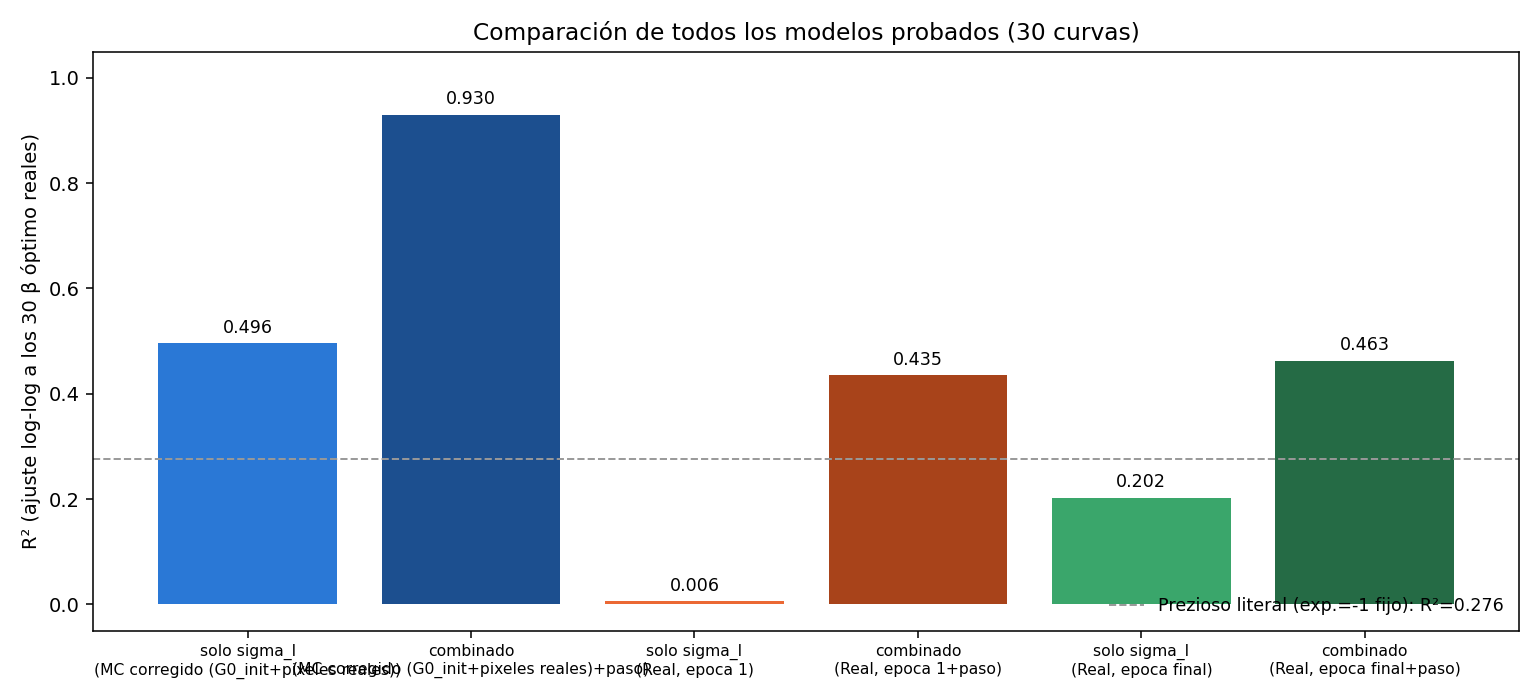
\includegraphics[width=0.9\textwidth]{comparacion_R2_todos_los_modelos_30curvas.png}
\caption{$R^2$ de los 6 modelos probados (3 fuentes de $\sigma_I$ $\times$
solo/combinado con \texttt{paso\_medio}), 30 curvas. La línea punteada es
Prezioso literal (exponente $-1$ fijo).}
\end{figure}

Igual que con 18 curvas: fijar el exponente en $-1$ ($\beta=\kappa/\sigma_I$,
la forma literal citada por Prezioso et al.\ de LeCun et al.) da
$R^2=0.276$ con la mejor fuente de $\sigma_I$ (MC corregido) —el $\kappa$
implicado varía $5.1\times$ entre curvas. Con las otras dos fuentes de
$\sigma_I$ (corriente real) el ajuste literal es directamente malo o
negativo ($R^2=-0.11$ y $R^2=-0.02$).

Dejando el exponente \textbf{libre} y agregando \texttt{paso\_medio\_pot}
como segunda variable, el modelo con \texttt{sigma\_I\_mc\_corregido} es,
por lejos, el mejor de los 6 probados: $R^2=0.930$, muy por encima de
cualquier variante con corriente real ($R^2\leq0.46$) —igual que con 18
curvas, usar la corriente ya entrenada (que depende circularmente del
propio $\beta$) empeora la predicción en vez de mejorarla.

\section{La fórmula final}

\begin{figure}[htb]
\centering
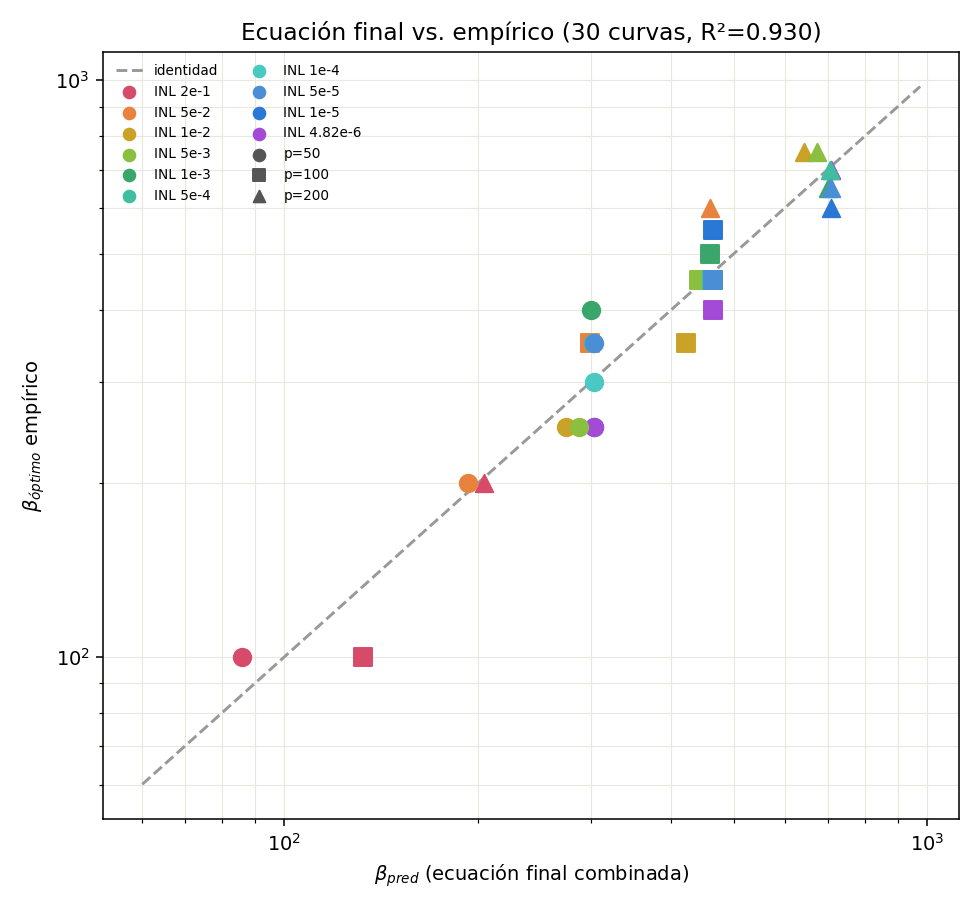
\includegraphics[width=0.62\textwidth]{ecuacion_final_vs_empirico_30curvas.png}
\caption{$\beta$ predicho por la ecuación final vs.\ $\beta$ óptimo
empírico, 30 curvas, $R^2=0.930$.}
\end{figure}

\begin{equation}
\beta_{\text{óptimo}} \approx 1.41\times10^{-8} \cdot \sigma_{I,MC}^{-3.00} \cdot \text{paso\_medio}^{-0.62}
\label{eq:final}
\end{equation}

con $\sigma_{I,MC}$ y \texttt{paso\_medio} en Siemens. $R^2=0.930$ sobre
las 30 curvas (ajuste log-log).

\begin{table}[htb]
\centering
\begin{tabular}{@{}lrr@{}}
\toprule
 & 18 curvas (reporte previo) & 30 curvas (este reporte) \\
\midrule
exponente de $\sigma_{I,MC}$ & $-3.06$ & $\mathbf{-3.00}$ \\
exponente de \texttt{paso\_medio} & $-0.61$ & $\mathbf{-0.62}$ \\
$R^2$ & 0.938 & $\mathbf{0.930}$ \\
\bottomrule
\end{tabular}
\caption{Comparación de coeficientes: 18 vs.\ 30 curvas.}
\end{table}

Los coeficientes son \textbf{prácticamente idénticos} al agregar 12 curvas
nuevas (4 valores de INL que no formaban parte del ajuste original,
incluyendo \texttt{5e-2} que cae justo en la zona de transición). Señal
fuerte de que la fórmula generaliza —no es un sobreajuste a las 6 curvas
originales.

\section{Validación práctica: ¿sirve para saltarse la búsqueda?}

\begin{figure}[htb]
\centering
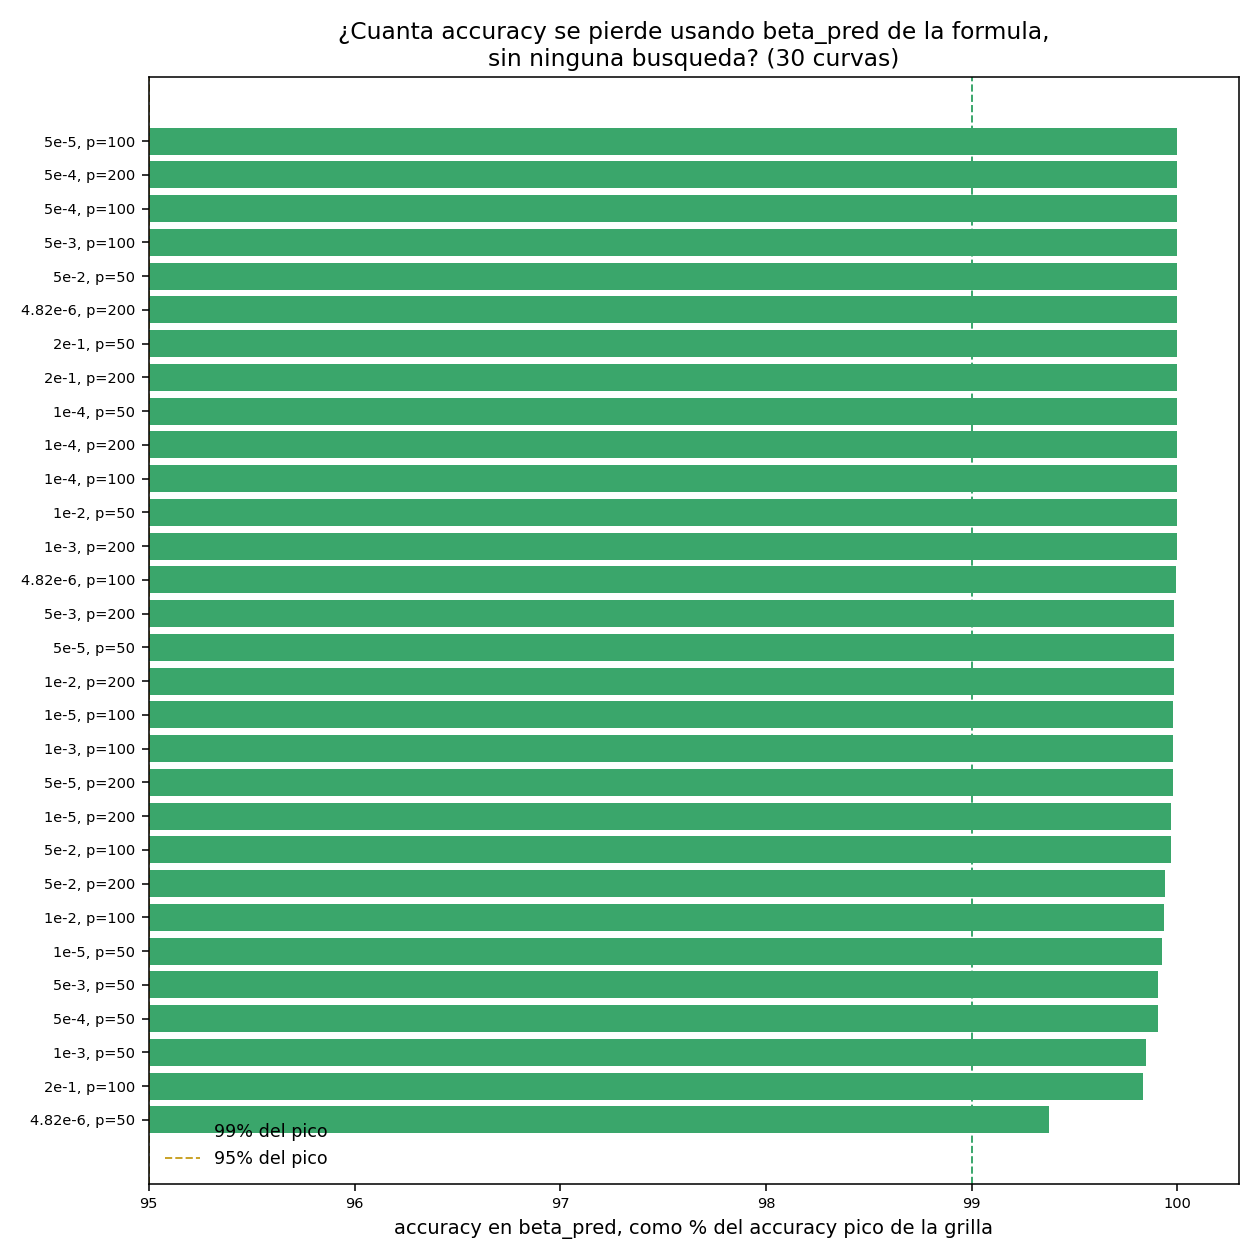
\includegraphics[width=0.85\textwidth]{formula_vs_grilla_real.png}
\caption{Accuracy en $\beta_{\text{pred}}$ como \% del pico real de cada
curva (grilla completa de 40 $\beta$), 30 curvas ordenadas.}
\end{figure}

Para cada curva: se calculó $\beta_{\text{pred}}$ con la
Ec.~\ref{eq:final} (sin entrenar nada), se buscó el punto de la grilla
real de 40 $\beta$ más cercano, y se comparó su accuracy contra el pico
real de esa curva completa —no una aproximación de meseta simétrica como
en el reporte de 18 curvas, sino la grilla real.

\textbf{Resultado: 30 de 30 curvas alcanzan $\geq$99\,\% de su accuracy
pico} (media 99.95\,\%, mínimo 99.38\,\% en \texttt{INL=4.82e-6, p=50})
usando $\beta_{\text{pred}}$ sin ninguna búsqueda —a pesar de que el error
de $\beta_{\text{pred}}$ contra $\beta_{\text{óptimo}}$ real llega hasta
$\pm$32\,\% en algunas curvas (Sección~5). Tiene sentido: las curvas
accuracy-vs-$\beta$ tienen un pico ancho (meseta), así que un error de
20--30\,\% en $\beta$ no cuesta casi nada de accuracy real.

\section{Errores por curva —dónde falla más la fórmula}

\begin{table}[htb]
\centering
\begin{tabular}{@{}lrrr@{}}
\toprule
curva & $\beta$ empírico & $\beta$ predicho & error \\
\midrule
\texttt{INL=2e-1, p=100}   & 100 & 132.5 & \textbf{+32.5\,\%} \\
\texttt{INL=1e-3, p=50}    & 400 & 300.0 & \textbf{-25.0\,\%} \\
\texttt{INL=5e-2, p=200}   & 600 & 459.8 & -23.4\,\% \\
\texttt{INL=1e-5, p=50}    & 250 & 303.5 & +21.4\,\% \\
\texttt{INL=4.82e-6, p=50} & 250 & 303.5 & +21.4\,\% \\
\texttt{INL=1e-2, p=100}   & 350 & 421.0 & +20.3\,\% \\
\multicolumn{4}{c}{\emph{(24 curvas restantes: entre -15\,\% y +18\,\%)}} \\
\bottomrule
\end{tabular}
\caption{Peores errores de predicción, 30 curvas. Tabla completa:
\texttt{resultados\_prezioso\_30curvas.csv}.}
\end{table}

Error absoluto porcentual: \textbf{media=11.5\,\%, mediana=11.7\,\%,
máximo=32.5\,\%} sobre las 30 curvas. Los peores casos se concentran en
$p=50$ (curva P/D más gruesa, \texttt{paso\_medio\_pot} más grande —el
término que más castiga la predicción) y en \texttt{INL=2e-1} (la curva
más no lineal, con la dinámica de entrenamiento más inestable, ver
\texttt{analisis\_distribucion\_softmax\_INL\_2e-1\_comparacion\_p/}
—tiene sentido que sea también donde la fórmula, que solo mira la curva
P/D antes de entrenar, tenga más dificultad).

\section{Conexión con los hallazgos de distribución de logits/softmax}

Esta fórmula predice $\beta$ óptimo \textbf{antes de entrenar}, a partir
solo de la curva P/D. Es distinta —y complementaria— del hallazgo de
\texttt{analisis\_distribucion\_softmax\_INL\_2e-1\_comparacion\_p/}: ahí
se vio que el desvío estándar de los logits \textbf{ya entrenados}
($\beta\cdot I$, modelo convergido) en el $\beta$ óptimo cae en una banda
angosta \emph{dentro de un mismo INL} (1.8--2.7 para \texttt{INL=2e-1},
3.5--6.4 para \texttt{INL=1e-2}) pero esa banda \textbf{no es universal
entre INL distintos}.

Esto es coherente con el resultado de esta sección: el exponente de
$\sigma_I$ en la fórmula es $-3$, no $-1$ (Prezioso literal asumiría
$\beta\cdot\sigma_I\approx\kappa$ constante) —el propio dato ya venía
diciendo que la relación entre $\beta$ óptimo y la dispersión de corriente
NO es tan simple. La fórmula de esta sección usa $\sigma_I$ de
\textbf{inicialización} con un exponente fuerte ($-3$) para compensar
exactamente esa no-linealidad; el hallazgo de logits post-entrenamiento la
confirma desde el otro extremo (después de entrenar, la ``banda sana'' de
dispersión de logits también depende del INL, no es una constante única).

\section{Limitaciones (heredadas del reporte de 18 curvas, sin resolver aún)}

\begin{itemize}
\item \textbf{N fijo.} Las 30 curvas comparten $N=784$ (fan-in de MNIST)
  —el exponente de $N$ en la ecuación teórica ($N^{-1/2}$) sigue sin poder
  testearse con esta data.
\item \textbf{Un solo dataset.} Fashion-MNIST ya está disponible
  (\texttt{X\_train\_mnist\_fashion.npy}) pero no se usó todavía.
\item \textbf{Grilla de $\beta$ de 40 puntos, espaciados de a 50.} El
  $\beta$ óptimo empírico contra el que se ajusta tiene ese error de
  resolución.
\item \textbf{Zona de transición INL incompleta.} \texttt{7e-2, 1e-1,
  1.3e-1, 1.6e-1} (jobs ya generados, \texttt{train\_job\_INL\_7e-2\_p\_50.sh}
  y afines, pero aún no corridos/bajados) llenarían el hueco entre
  \texttt{5e-2} y \texttt{2e-1}.
\item \textbf{Ajuste in-sample.} Los $R^2$ se calculan sobre las mismas 30
  curvas usadas para ajustar los coeficientes. La estabilidad de los
  coeficientes al pasar de 18$\to$30 curvas (Sección~3) es la mejor
  evidencia disponible de que no es sobreajuste, pero no reemplaza una
  validación real con datos no usados en el ajuste.
\end{itemize}

\section{Recomendación (sin cambios respecto del reporte de 18 curvas, ahora con más evidencia)}

Igual que antes: \textbf{no reemplazar \texttt{search\_best\_beta()} por
la fórmula en modo ``un solo paso, sin verificar''}. Usarla como
\textbf{pre-filtro barato}: calcular $\beta_{\text{pred}}$ (sin entrenar
nada) y correr \texttt{search\_best\_beta()} en una ventana angosta
alrededor ($\beta_{\text{pred}}\times[0.5,2]$, 5--7 puntos) en vez de la
grilla completa (1--1950, 40 puntos) —ahorro de cómputo de $\sim$5--8$\times$
sin perder la garantía de una búsqueda real. La evidencia de este reporte
(30/30 curvas $\geq$99\,\% del pico, con la grilla REAL) es más fuerte que
la del reporte de 18 curvas, pero sigue siendo evidencia sobre un único
régimen (SP, $N=784$, MNIST) —no una garantía general.

\section{Archivos generados}

\begin{itemize}
\item \texttt{reconstruir\_corrientes\_30curvas.py} $\to$
  \texttt{resultados\_30curvas.csv}, \texttt{trayectorias\_std\_30curvas.png},
  \texttt{comparacion\_sigma\_fuentes\_30curvas.png}.
\item \texttt{probar\_prezioso\_y\_regresiones\_30curvas.py} $\to$
  \texttt{resultados\_prezioso\_30curvas.csv},
  \texttt{coeficientes\_todos\_los\_modelos\_30curvas.csv},
  \texttt{prezioso\_literal\_vs\_empirico\_30curvas.png},
  \texttt{comparacion\_R2\_todos\_los\_modelos\_30curvas.png},
  \texttt{ecuacion\_final\_vs\_empirico\_30curvas.png}.
\item \texttt{evaluar\_formula\_en\_grilla\_completa.py} $\to$
  \texttt{evaluacion\_formula\_en\_grilla.csv}, \texttt{formula\_vs\_grilla\_real.png}.
\item \texttt{reporte\_formula\_beta\_optimo\_30curvas.md} —versión
  Markdown de este mismo reporte.
\end{itemize}

\end{document}
